\section{Communication Filtering}\label{sec:communicationFiltering}
The GoT system yields the vehicle's position throughout time. However, since this system utilizes ultrasound waves to register positions in space, it can be distorted by interferences and objects on the wave path. It is therefore required to eliminate the big jumps in positions, that could occur in the GoT system, before sending them to the vehicle, see requirements in \chapref{Requirements}.

Since the vehicle cannot run faster than \si{3,0\ m \cdot s^{-1}}, it is possible to define a certain range of positions for a defined time interval. The range is defined as a circle, with the a radius as large as the assumed maximum velocity, set to \si{3,0\ m.s^{-1}}, multiplied with the measured time interval. An example with a \SI{0,1}{s} time interval is given on \figref{GoTFilterSimple}.
%
\begin{figure}[H]
  \centering
  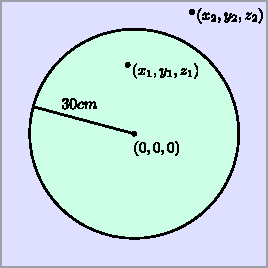
\includegraphics[scale=1.3]{figures/GoTFilterSimple.pdf}
  \caption{Range of possible positions for a maximum speed of \si{3,0\ m \cdot s^{-1}} during a \SI{0,1}{} second interval}
  \label{GoTFilterSimple}
\end{figure}\vspace{-5mm}
%
If the position at a given time, \si{t_0} is \si{(0,0,0)}, the coordinates at the next measurement time, $\text{t}_1 = \text{t}_0+\SI{0,1}{s}$, should stay within a \SI{30}{cm} radius of the first position.

To ensure the fact that no position jumps is sent to the vehicle, its velocity is measured from the two last sets of coordinates and the sampling time of the GoT system (\SI{100}{ms}, see \secref{GoTDescription}), see \eqref{eq:velocityGoTCalc}.
\begin{flalign}
\eq{v}{\frac{\sqrt{(X_{2} - X_{{1}})^2 + (Y_{2} - Y_{{1}})^2 + (Z_{2} - Z_{{1}})^2}}{\Delta T}}\unit{m \cdot s^{-1}}
\label{eq:velocityGoTCalc}
\end{flalign}
\hspace{6mm} Where:\\
\begin{tabular}{p{1cm}lll}
  &\si{v}                   & is the velocity of the vehicle                      &\unitWh{m \cdot s^{-1} }\\
  &\si{(X_{2},Y_{2},Z_{2})}   & is the the last set of measured coordinates         &\unitWh{m}\\
  &\si{(X_{1},Y_{1},Z_{1})}   & is the the second last set of measured coordinates  &\unitWh{m}\\
  &\si{\Delta T}            & is the sampling time                                &\unitWh{s}\\
\end{tabular}

Whenever a calculated velocity is greater than the limit of \si{3,0\ m \cdot s^{-1}}, the newest set of coordinates is completely discarded. To calculate the newest velocity afterwards, the previous position, that was not discarded, and the newly measured position are taken, and the sampling time is extended by \si{100\ ms}, until a velocity under the limit is measured. When the velocity is under the limit again, the time interval is set to the default value again.

However, if the GoT is correctly calibrated and the vehicle's environment is clear of interfering obstacles, the distributions will occur rarely.

The communication protocol has been designed to be able to disregard incorrect packages transmitted from the computer. Furthermore a filter has been implemented to ensure large distortion occurring in the GoT system, can be handled and filtered. This should fulfill the requirements set to the communication in \secref{Requirements}.